\textbf{Seats}
\begin{enumerate}
    \item 8 mins: Intro slides \par
    \item 20 mins: Finish Example 6.1.1 \par
    \textbf{Check piazza}
    \item 34 mins: Finish Example 6.1.2 \par
    \textbf{Check piazza}
    \item 50 mins: Introduce Example 6.2.1 \par
    \textbf{Check piazza}
\end{enumerate}
\textbf{Seats}

\vspace{10mm}
\textbf{Example 6.1.1}

Multiple-choice quiz?
\begin{itemize}
\item First-order
\item Second-order
\item Fifth-order
\end{itemize}

\vspace{10mm}
\textbf{Example 6.1.2}

First, show that 
\begin{align*}
A = \frac{1}{C e^{k_{AB} t} - 1} = \left(C e^{k_{AB} t} - 1\right)^{-1}
\end{align*}
is a solution. Differentiate the solution using the chain rule
\begin{align*}
\frac{{\rm d} A}{{\rm d} t} = - \frac{ k_{AB} C e^{k_{AB} t}}{ \left(C e^{k_{AB} t} - 1\right)^{2}}
\end{align*}
Now, calculate the RHS of the differential equation
\begin{align*}
-k_{AB}A(A+1) &=  -k_{AB} \frac{1}{C e^{k_{AB} t} - 1} \left(1 + \frac{1}{C e^{k_{AB} t} - 1} \right) \\
&= -k_{AB} \frac{1}{C e^{k_{AB} t} - 1} \frac{C e^{k_{AB} t} - 1 + 1}{C e^{k_{AB} t} - 1} \\
&=  - \frac{ k_{AB} C e^{k_{AB} t}}{ \left(C e^{k_{AB} t} - 1\right)^{2}}.
\end{align*}
To apply the initial condition, substitute in $t=0$, which gives $A(0) = 1/(C-1) = 1$, and so $C=2$.


\vspace{10mm}
\textbf{Example 6.2.1}

To draw the solution
\begin{itemize}
\item Find the stationary points. ${\rm d}y/{\rm d} x = 0$ when $x+y=0$ so $y=-x$. So draw horizontal arrows along the line $y=-x$.
\item The gradient increases as both $x$ and $y$ increase, so draw arrows pointing down and to the right below/left of $y=-x$ and pointing up and to the right above/right of $y=-x$.
\item Note that at $y = -x - 1$ the arrows have gradient $-1$, so they will carry on parallel to the stationary point. (Students wouldn't be expected to find this unaided in an exam). 
\item Draw solutions starting at various points from $x=0$. If we choose $y<-1$ we see the solution just keeps decreasing. For $y=-1$ it runs parallel to the stationary point. For $-1 < y < 0$ the line begins decreasing and crosses the line $y=-x$ to end up increasing. For $x>0$ the solution is always increasing.
\end{itemize}

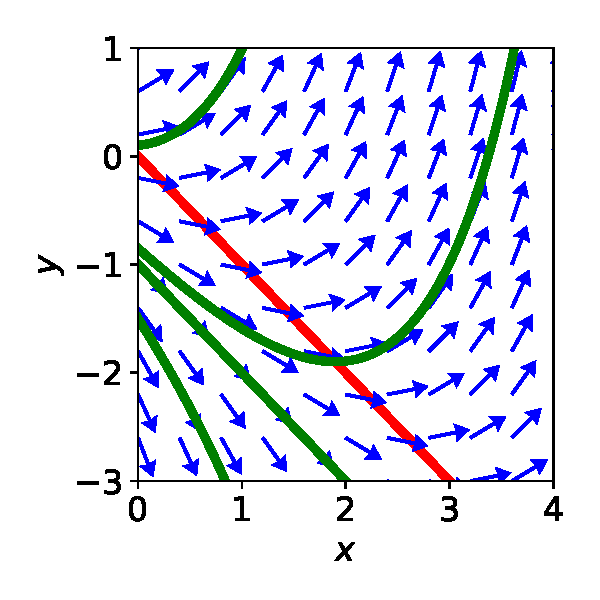
\includegraphics{Figures/ex_621.pdf}
